\chapter{The TR-\textit{ic}OS setup at the ESRF: time-resolved microsecond UV-Vis absorption spectroscopy on protein crystals}\label{chap:TR-icOS}

\vspace{10mm}

The technique of time-resolved macromolecular crystallography (TR-MX) has recently been rejuvenated at synchrotrons, resulting in the design of dedicated beamlines. Using pump-probe schemes should make the mechanistic study of photoactive proteins and other suitable systems possible with time resolutions down to microseconds. To identify relevant time delays, time-resolved spectroscopic experiments directly performed on protein crystals are often desirable. To this end, an instrument has been built at the \textit{ic}OS Lab (\textit{in crystallo} Optical Spectroscopy Laboratory) at the European Synchrotron Radiation Facility using reflective focusing objectives with a tuneable nanosecond laser as a pump and a microsecond xenon flash lamp as a probe, called the TR-\textit{ic}OS (time-resolved \textit{ic}OS) setup. Using this instrument, pump-probe spectra can rapidly be recorded from single crystals with time delays ranging from a few microseconds to seconds and beyond. This can be repeated at various laser pulse energies to track the potential presence of artefacts arising from two-photon absorption, which amounts to a power titration of a photoreaction. This approach has been applied to monitor the rise and decay of the M state in the photocycle of crystallized bacteriorhodopsin and showed that the photocycle is increasingly altered with laser pulses of peak fluence greater than 100 mJ.cm\textsuperscript{-2}, providing experimental laser and delay parameters for a successful TR-MX experiment.


\section{Introduction}
Time-resolved macromolecular crystallography (TR-MX) was successfully developed in the 1990s, taking advantage of the polychromatic, intense single X-ray pulses of third-generation synchrotron storage rings \parencite{moffatLaueDiffractionTimeresolved2019}. The experiments were performed using a pump-probe scheme (Fig. \ref{fig:TRicOS_pumpprobe}) with a picosecond optical laser as the pump. The maximum time resolution of these experiments eventually reached the \textasciitilde100 ps duration of a single X-ray bunch. Laue TR-MX produced remarkable molecular movies of the photolysis and rebinding reaction of carbon monoxide in complex with myoglobin \parencite{schotteWatchingProteinIt2003} and of the photocycle of the photoactive yellow protein (PYP) \parencite{jungVolumeconservingTransCis2013}. However, the technique remained limited to biological systems which could yield low-mosaicity crystals of significant size (hundreds of micrometres in at least two directions) and for which the photoreaction could be repeatedly cycled without compromising the diffraction quality of the crystals.
The development of hard X-ray free-electron lasers (XFELs) revived the field of TR-MX \parencite{brandenAdvancesChallengesTimeresolved2021}. The duration of the very intense X-ray pulses that they produce can be as low as a few femtoseconds (resulting in the technique being called TR-SFX, ‘time-resolved serial femtosecond crystallography), but in contrast to Laue TR-MX the limitation on the time resolution is the pulse duration of the pumping optical laser (\textasciitilde100 fs; Fig. \ref{fig:TRicOS_pumpprobe} Fig. \ref{fig:TRicOS_pumpprobe}). The principle of recording one single diffraction image from a given sample at an XFEL before it is destroyed called for the use of a large number of micrometre-sized crystals (‘microcrystals’) and led to the development of serial crystallography (SX). It was soon realized that SX could be performed at third-generation synchrotrons, eventually leading to TR-SMX (serial millisecond crystallography; \cite{noglyLipidicCubicPhase2015}) and TR-SSX (serial synchrotron X-ray crystallography; \parencite{diederichsSerialSynchrotronXRay2017}). In particular, TR-SSX was applied to microbial rhodopsins, such as bacteriorhodopsin, to reach 5 \textmu s time resolution \parencite{weinertProtonUptakeMechanism2019} and, very recently, to a xenorhodopsin with 500 \textmu s time resolution \parencite{kovalevMechanismsInwardTransmembrane2023}.
\begin{figure}[H] %bt!]
    \centering
    \noindent 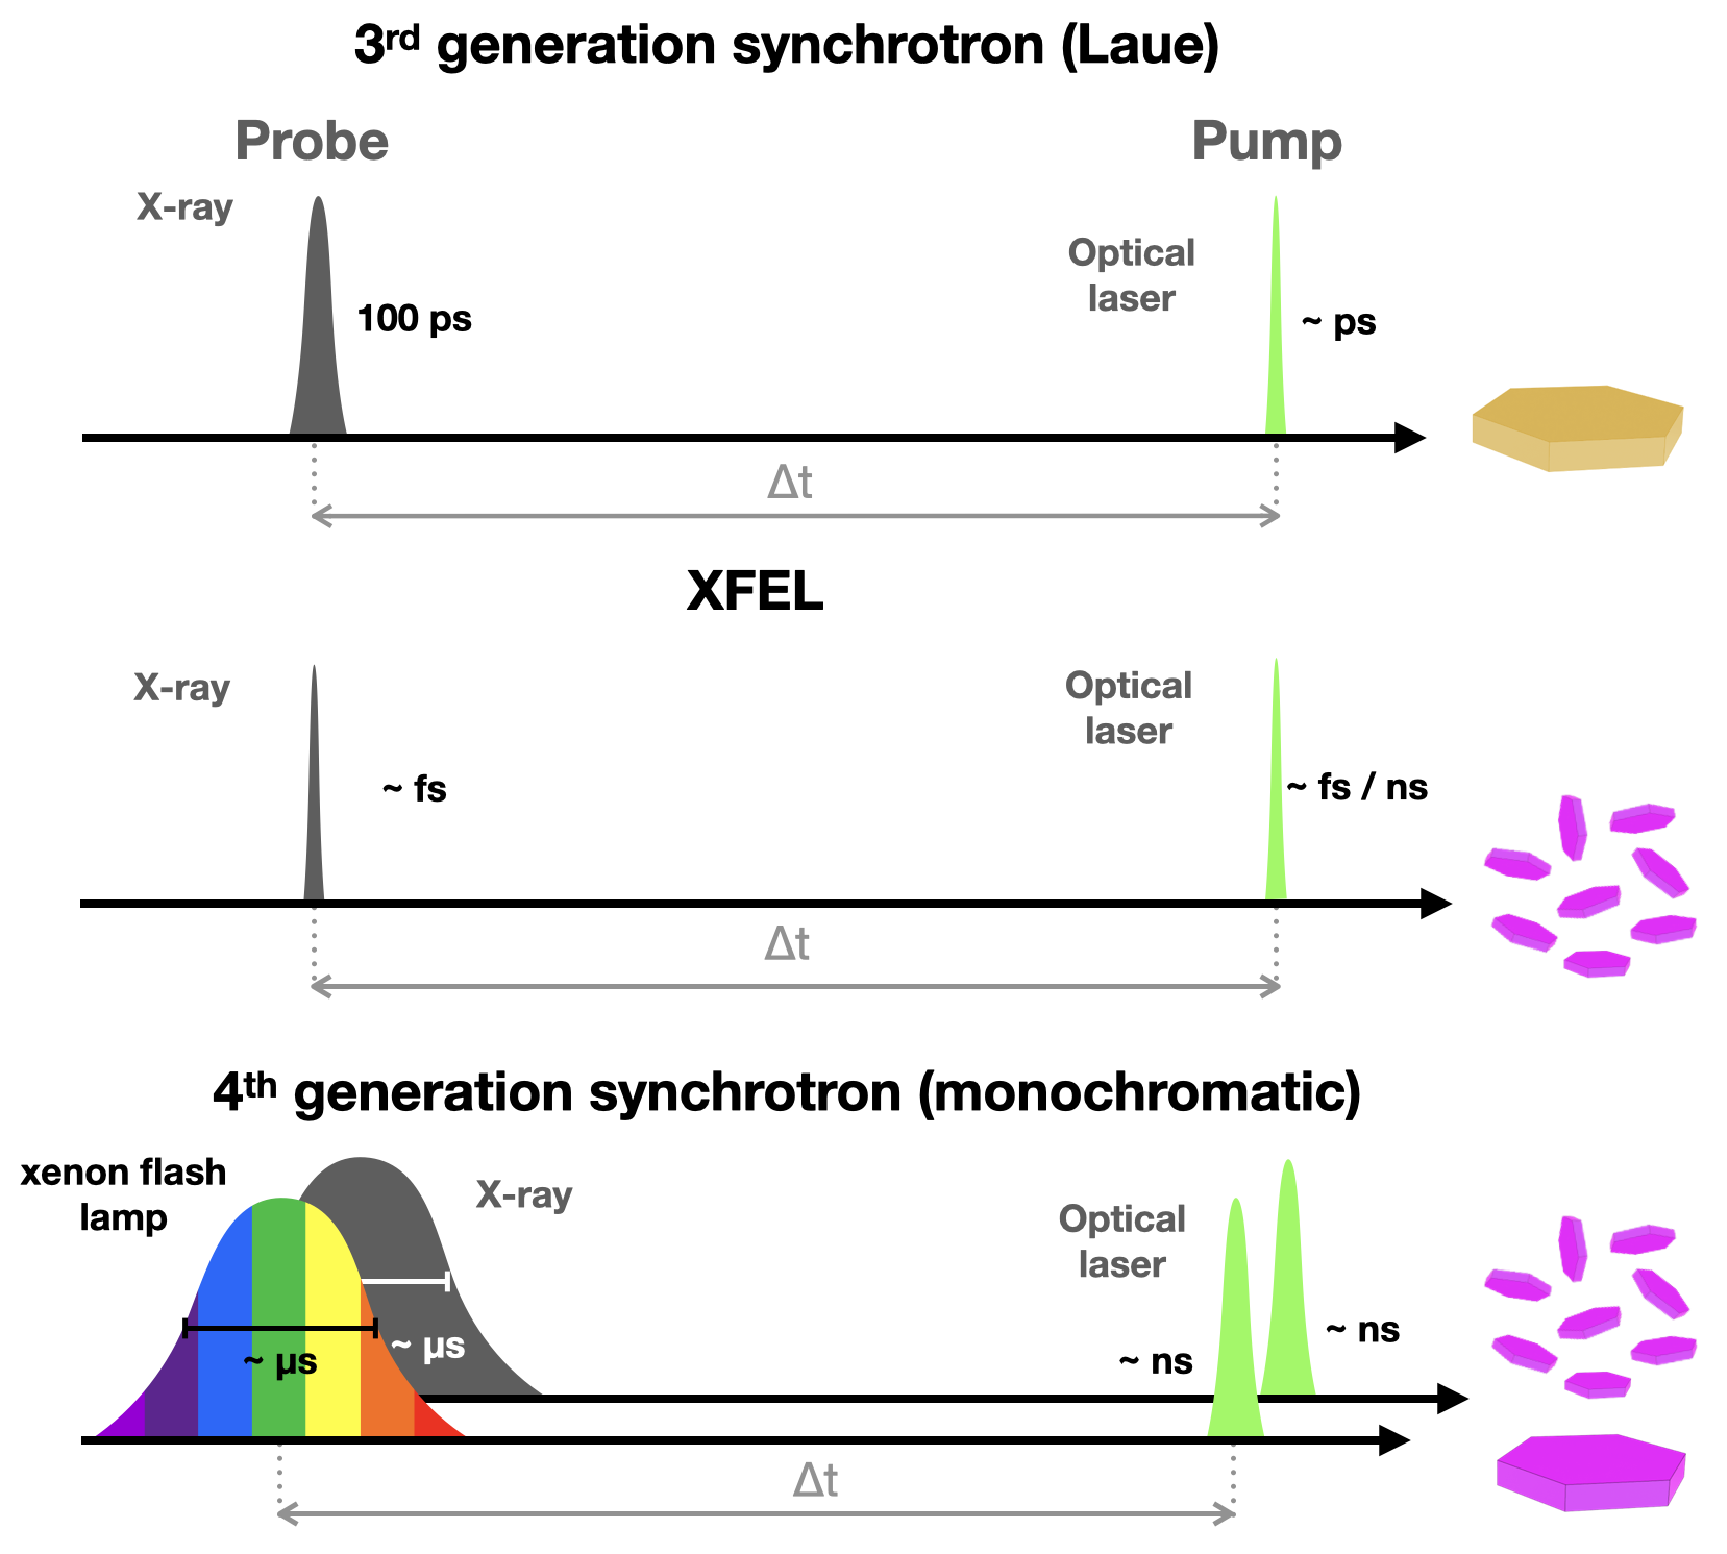
\includegraphics[width=\textwidth]{images/Spectroscopy/TRicOS_Fig1.pdf}
    \hfill
    \caption{Schematics showing the principles of a time-resolved pump-probe experiment using picosecond Laue diffraction on single crystals at third-generation synchrotrons (top), SFX at XFELs on microcrystals (middle) and SSX at fourth-generation synchrotrons (bottom). The optical laser pump signal is shown in green, X-ray pulses in grey and white-light pulses in rainbow colours. The crystal colours correspond to the prototypal photoactive yellow protein (PYP) studied by Laue diffraction and to bacteriorhodopsin for XFEL and monochromatic synchrotron diffraction. The microsecond X-ray pulse in the lower panel is shown for simplicity with a Gaussian profile when it should have a trapezoidal shape since it is generated using a rotating chopper.}
    \label{fig:TRicOS_pumpprobe}
\end{figure}
Over the last decade, third-generation synchrotrons have planned the design and construction of significantly improved machine layouts leading to much higher brilliance and coherence of the X-ray beams produced. The European Synchrotron Radiation Facility (ESRF) in Grenoble, France and MAX IV in Lund, Sweden are the first two fourth generation synchrotrons to have carried out the construction of specific TR-SSX beamlines, taking advantage of the much higher brilliance to produce large-bandwidth monochromatic microsecond pulses. ID29-SMX at the ESRF is the first such beamline (\href{https://www.esrf.fr/id29}{esrf.fr/id29} and will be followed by MicroMAX at MAX IV (\href{https://www.maxiv.lu.se/micromax}{maxiv.lu.se/micromax}).
Photoreactions of proteins do not necessarily proceed in the crystalline state exactly as in solution (see, for instance, the identification of an intermediate state that exists in the \textit{in crystallo} photocycle of PYP but not in the photocycle in solution; \cite{konoldConfinementCrystalLattice2020}), hence it is highly desirable to perform spectroscopic experiments on crystalline samples prior to any TR-MX experiment. This helps to validate the rise and decay of various intermediates so that relevant time points can be chosen (see for instance, the build-up of the late L and M intermediate states in the photocycle of bacteriorhodopsin; \cite{nangoThreedimensionalMovieStructural2016}). Moreover, it has recently been pointed out that the absorption of multiple photons from the pump laser could affect the photoreaction and potentially lead to artefacts in the interpretation of structural intermediates \parencite{millerThreedimensionalViewUltrafast2020, barendsInfluencePumpLaser2024,bertrandStructuralEffectsHigh2024}. Power-titration spectroscopic experiments prior to the diffraction experiment should help to identify these potential artefacts.
In order to prepare and support TR-SSX experiments, we have built a setup that is capable of measuring time-resolved UV–Vis absorption spectra on macromolecular crystals on the microsecond-to-second timescale. The TR-\textit{ic}OS instrument is located in the \textit{ic}OS Lab at the ESRF (\href{https://www.esrf.fr/icOS}{esrf.fr/\textit{ic}OS}; \cite{vonstettenCrystalloOpticalSpectroscopy2015}) beside the new serial crystallography beamline ID29-SMX. The \textit{ic}OS Lab groups together a number of instruments that can be used to perform various types of spectroscopies (UV–Vis absorption, fluorescence emission, Raman) on crystals at cryogenic or room temperature, either in a static or slow-time-resolved (time resolution of tens of milliseconds) manner. TR-\textit{ic}OS has been developed to identify spectroscopic transitions occurring \textit{in crystallo} for a given photoactivatable biological system upon nanosecond light activation. The setup has two main purposes in future TR-MX experiments: it will facilitate the identification of interesting delays and it will provide complementary information to cross-validate diffraction data.



\section{Experimental procedure}


Two types of samples can be loaded: either single crystals obtained in a crystallization plate or slurries of microcrystals obtained in batches. In the former case, 2 ml of the crystallization mother liquor is loaded into one well of the sample holder and a handful of crystals are manually transferred into this drop using a crystallization loop. In the latter case, the microcrystal slurries are diluted several times and 2 ml of each resulting solution is loaded into a different well of the sample holder. The microscope objectives are first used to locate a suitable crystal upon iterative horizontal translation of the sample stage. The sample Z position is then adjusted by vertically translating the stage until a sharp image is obtained with the camera using the reflective objective, meaning that both the laser and flash-lamp focal spots are positioned at the top surface of the crystal. However, having inserted a large object between the two reflective objectives with a refractive index different from that of air, the focal volumes (of \textasciitilde20 mm thickness) of both objectives no longer match. Thus, the bottom objective is then translated along the Z-axis until the transmitted light signal is maximized. From then onwards, only minimal recentring is needed to move from one crystal to the other within a given well of the sample holder. Reference and dark spectra are first recorded in the vicinity of the crystal of interest and are used for all subsequent \textit{ic}AS spectra. A typical pump-probe experiment starts with the recording of ground-state spectra. The OPO shutter is then manually opened and a series of pump-probe spectra can be obtained by varying the delay between the nanosecond laser and xenon flash-lamp pulses in the CITY module terminal. The resulting pump-probe spectra series corresponds to a given laser pulse energy and can be repeated at different energies by rotating the energy-attenuating wheel.

\section{Results}


We used the membrane proton pump bacteriorhodopsin from \textit{Halobacterium salinarum} (BR) as a benchmark photoactive protein for our setup. The photocycle of BR in its native environment, the so-called purple membrane, develops over many orders of magnitude in time from the spectroscopic intermediate states I (rise time of \textasciitilde200 fs), J (\textasciitilde450 fs), K (\textasciitilde4 ps), L (\textasciitilde1 \textmu s), M1 (\textasciitilde40 \textmu s), M2 (\textasciitilde350 \textmu s), N (\textasciitilde5 \textmu s) and, finally, O (\textasciitilde5 \textmu s), as determined by various spectroscopic methods \parencite{doigPicosecondTimeresolvedResonance1991, neutzeBacteriorhodopsinHighresolutionStructural2002}. The whole photocycle is completed within \textasciitilde20 m s and is reversible in crystals. However, the rise times of these intermediate states vary between the purple membrane and a crystalline environment \parencite{efremovTimeResolvedMicrospectroscopySingle2006, weinertProtonUptakeMechanism2019}; thus, UV–Vis absorption spectroscopy experiments directly performed on crystals are required to determine the time points of interest in TR-MX experiments on BR crystals. The time resolution of our instrument (2 \textmu s) is suited to probe the buildup of late intermediates, starting with the M1 state.
Crystals of BR, expressed and purified as described by \cite{gordeliyCrystallizationLipidicCubic2003}, were crystallized as described by \cite{borshchevskiyTrueatomicresolutionInsightsStructure2022}, resulting in hexagonal plates with dimensions of \textasciitilde50–200 \textasciitilde 50–200 \textasciitilde 10–20 mm3 (Fig. \ref{fig:TRicOS_results}a). Crystals were placed in the sample holder after manual harvesting in the lipidic cubic phase (LCP) using a standard MiTeGen loop (\href{https://www.mitegen.com}{www.mitegen.com}).
To identify the time range during which occupancy of the M state is maximal, we recorded \textit{ic}AS spectra with pump-probe delays ranging from 3 \textmu s to 1 s (Fig. \ref{fig:TRicOS_results}a). A given experiment is performed at a certain pulse energy (75 mJ.cm\textsuperscript{-2}; Fig. \ref{fig:TRicOS_results}a). To assess the complete reversibility of the photoreaction and thus the possibility of performing several time-resolved measurements on the same crystal, a ground-state spectrum is recorded prior to a pump-probe transient spectrum. The lack of bleaching of the photoactive protein can be verified by the iterative superimposition of successive ground-state spectra. The build-up and decay of the M state can be visualized by monitoring the absorbance at 415 nm. As expected, the M state is already present in the crystal 3 \textmu s after light excitation, and its occupancy is maximal between 100 \textmu s and 1 ms (black trace in Fig. \ref{fig:TRicOS_results}b). The build-up/ decay profile matches published data recorded on BR crystals \parencite{efremovTimeResolvedMicrospectroscopySingle2006}.
This experiment was repeated at various laser-pulse energies, thus producing a power titration (or, more rigorously, a peak-fluence titration) of the M-state build-up and decay profile. The peak fluence was varied from 18 to 633 mJ.cm\textsuperscript{-2} (calculations were performed as in \cite{nasskovacsThreedimensionalViewUltrafast2019}). The resulting profiles can be divided into three groups. The first, grouping seven experiments with fluences between 18 and 75 mJ.cm\textsuperscript{-2}, resembles the profile determined by \cite{efremovTimeResolvedMicrospectroscopySingle2006}, except that the ratio of the respective M-state amplitudes at 10 \textmu s and 300 \textmu s (close to the maximum M-state occupancy) is \textasciitilde60\% in the former and \textasciitilde30\% in the latter. The second groups three experiments with fluences between 81 and 151 mJ.cm\textsuperscript{-2}, for which the profile is distorted with a 10 \textmu s:300 \textmu s amplitude ratio nearing 100\%. Finally, the third group (between 163 and 633 mJ.cm\textsuperscript{-2}) exhibits a profile that clearly deviates from the expected profile, with a monotonous decay from a maximum occupancy at 3 \textmu s.

\begin{figure}[H] %bt!]
    \centering
    \noindent 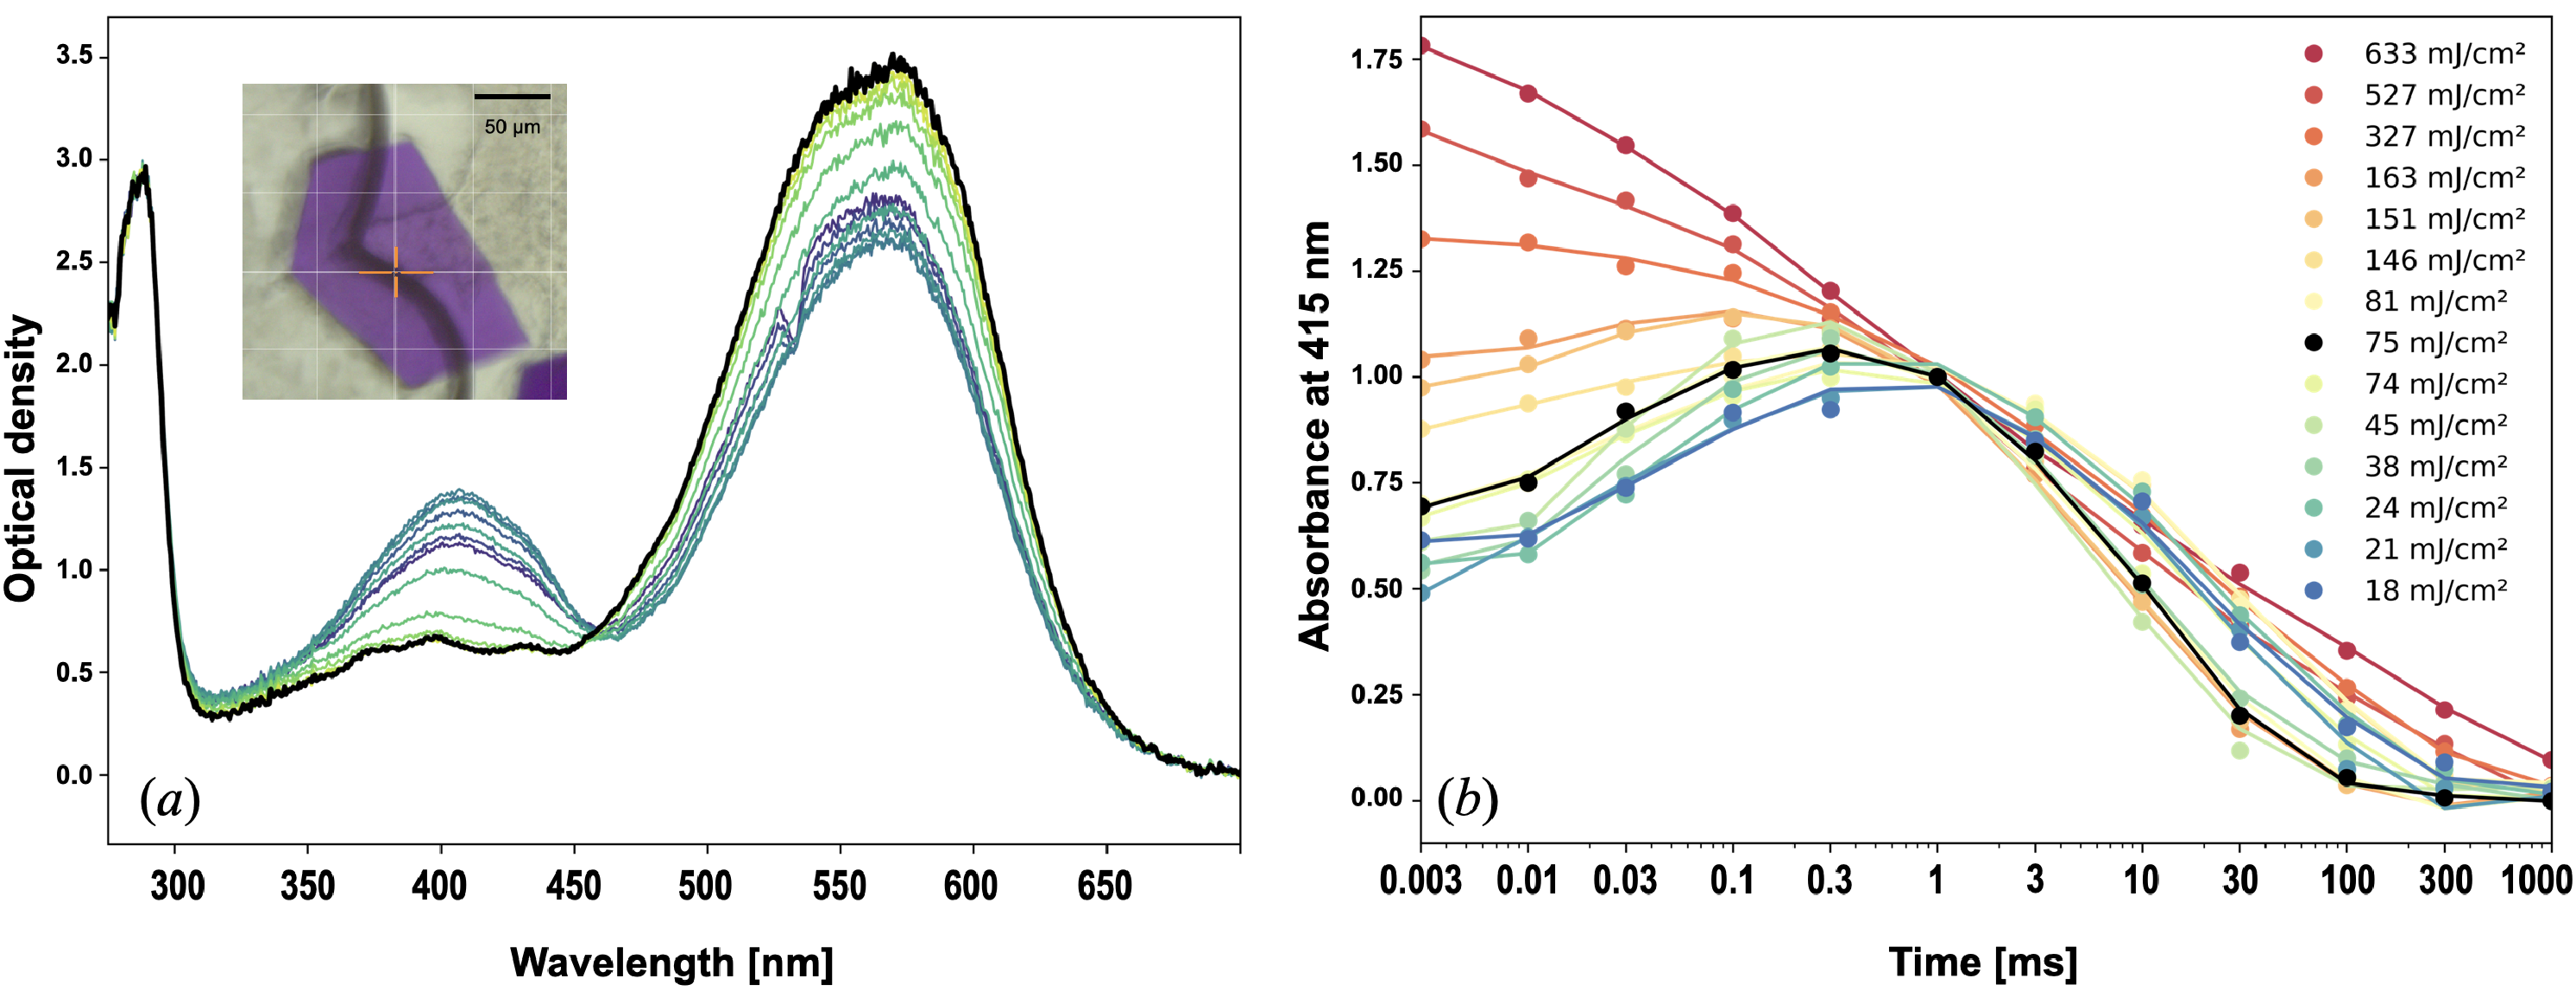
\includegraphics[width=\textwidth]{images/Spectroscopy/TRicOS_Fig8.pdf}
    \hfill
    \caption{(\textit{a}) Time-resolved series of \textit{ic}AS spectra obtained on a single BR crystal (see insert) with delays varying logarithmically between 3 \textmu ss and 1 s (purple to blue to green). The initial ground-state spectrum is shown as a thick black line. The excitation wavelength is 532 nm and the pulse energy is 75 mJ.cm\textsuperscript{-2} at the sample position. (\textit{b}) Power titration of the M-state time evolution. For each spectrum of the time series recorded at a given fluence, the optical density at 415 nm (OD\textsubscript{415}, from which the OD\textsubscript{415} of the ground state has been subtracted) is plotted as a function of time. The resulting profiles have been scaled to each other using the OD\textsubscript{415} value at 1 ms. The black trace corresponds to the profile of the experiment depicted in (\textit{a}).}
    \label{fig:TRicOS_results}
\end{figure}

These results suggest that the fluence used for the first profile group corresponds to a functional photocycle in the crystals and that increasing fluences lead to the build-up of an artefactual M state, which, we postulate, could well correspond to direct chromophore deprotonation upon multiphoton absorption. The population of this artefactual M state adds up to that of the expected M state at early time points (the second group) and then eventually dominates (the third group). This suggests limiting peak fluences in diffraction experiments to values below 100 mJ.cm\textsuperscript{-2}. Fortunately, several recent TR-MX experiments performed on BR at XFELs and synchrotrons have been conducted using fluences in this regime. Ultrafast intermediate states I to K have been probed at 42 mJ.cm\textsuperscript{-2} \parencite{noglyRetinalIsomerizationBacteriorhodopsin2018} and 69 mJ.cm\textsuperscript{-2} \parencite{nasskovacsThreedimensionalViewUltrafast2019} (these values were calculated without taking into account scattering from the carrying medium). Later intermediate states K to M have been studied at 110 mJ.cm\textsuperscript{-2} \parencite{nangoThreedimensionalMovieStructural2016}. Finally, the large structural changes of the late intermediate states M2 to N have been visualized at 50 mJ.cm\textsuperscript{-2} (recalculated from \cite{weinertProtonUptakeMechanism2019}). Of note, the early study focused on \textit{in crystallo} spectroscopic characterization \parencite{efremovTimeResolvedMicrospectroscopySingle2006} reported a peak fluence of 3 mJ.cm\textsuperscript{-2} and thus constitutes the \textit{in crystallo} study of the BR photocycle with the lowest reported fluence.  While the fluence of the Nango study may appear to be slightly higher than the identified threshold, the loss of photons via scattering at the surface, and through the LCP microjet, likely led to an effective fluence below this threshold. Overall, these results confirm the proposition by Brändén and Neutze that multiphoton regimes may not systematically deviate from the single-photon regime and that they could be used to maximize crystallographic occupancy \parencite{brandenAdvancesChallengesTimeresolved2021}.

\section{Perspectives}

Fourth-generation synchrotrons have reached unprecedented brilliance thanks to their low emittance, offering the possibility of intense monochromatic microsecond X-ray pulses. This, coupled with the recent revival of TR-MX at synchrotrons, has triggered the design of dedicated beamlines, starting with ID29 at the ESRF and MicroMAX at MAX IV, at which microsecond time resolution can be achieved. Other existing state-of-the-art beamlines already performing millisecond time-resolution TR-MX, such as TREXX at PETRA III \parencite{schulzHitandreturnSystemEnables2018}, I24 at Diamond Light Source \parencite{baxterObservationCationChromophore2022} and X06SA at the Swiss Light Source \parencite{weinertProtonUptakeMechanism2019}, will likely be upgraded so they can also achieve microsecond time resolution. This should bolster the field of dynamic photobiology as studied by TR-MX. In order to best prepare diffraction experiments on photoactive proteins, prior characterization of crystals by time-resolved spectroscopy is essential for the identification of time points of interest and for optimization of the choice of laser fluence. In particular, the latter should help to maximize intermediate-state occupancy in the diffraction data, while preventing or minimizing the possibility of artefactual photoreactions. We have built the TR-\textit{ic}OS instrument to serve these purposes. It is also meant to evolve, for instance, to probe flowing microcrystals in a suitable microfluidic device and, using photocaged substrates or cofactors, to exploit non-photoactive proteins in which the UV–Vis absorption properties of a certain chemical group evolve with time.

\section{Acknowledgements}

Thomas Vigouroux is acknowledged for his contribution to software writing at an early stage of the project. Kirill Kovalev, Manuel Maestre-Reyna, Po-Hsun Wang, Anaïs Chrétien, Robin Schubert and Valerie Panneels are acknowledged for help and discussion during instrument commissioning. VG highly appreciates support within the framework of Commissariat à l’Energie Atomique et aux Energies Alternatives (Institut de Biologie Structurale) - HelmholtzGemeinschaft Deutscher Forschungszentren (Forschungszentrum Jülich).


\chapter{The \textit{in crystallo} Optical Spectroscopy toolbox}\label{chap:toolbox}

\textbf{Abstract }Over the last ten years, there has been a surge in the demand for \textit{in crystallo} optical spectroscopy (\textit{ic}OS), as optical spectroscopy is one of the few biophysical characterisation method applicable to both solutions and crystals of proteins. Historically, \textit{ic}OS has been used to compare the state of proteins in crystals and in solution, and to assess their functionality by determining the redox state of metal ions, cofactors, or chromophores. The recent rejuvenation of time-resolved crystallography experiments has sparked a renewed interest in optical spectroscopy as a bridge between kinetic studies in solution and in the crystalline state. \textit{ic}OS can be defined as the ensemble of spectroscopic techniques in the UV-Visible-infrared range that can be applied to crystals. It has also been instrumental in understanding specific X-radiation damage to redox sensitive parts of proteins. Spectra recorded from crystals are affected by crystal orientation, shape, or position due to various optical phenomena. Fortunately, these can be modelled and corrected. The \textit{ic}OS Lab, at the ESRF, specialises in the recording of UV-Vis absorption, fluorescence emission and Raman spectra from protein crystals. Here we present a suite of utilities that streamline the analysis and correction of UV-Vis absorption \textit{ic}OS data, encased in a graphical interface. This was originally developed for the \textit{ic}OS Lab at the European Synchrotron Radiation Facility (ESRF) but is available as a standalone package, with the aim to make \textit{ic}OS more accessible.

\section{Introduction}

\textit{In crystallo} optical spectroscopy (\textit{ic}OS) was born of the need for the first protein crystallographers to assess how comparable their crystal structures were to the conformations of biomolecules in solution \parencite{mozzarelliProteinFunctionCrystal1996}. This validation was achieved by performing kinetic assays using UV-Vis absorption spectroscopy (AS) on a suspension of crystals instead of a protein solution. AS studies conducted on slurries of crystals within their mother liquor validated that ribonuclease S \parencite{doscherActivityEnzymeCrystalline1963}, alpha-chymotrypsin \parencite{kallosCatalyticActivityChymotrypsin1964}, Carboxypeptidase-A \parencite{quiochoEnzymicBehaviorCarboxypeptidaseA1966}, as well as many other enzymes both at physiological and sub-zero temperatures \parencite{finkFormationStableCrystalline1976,makinenReactivityCryoenzymologyEnzymes1977}, were active in the crystalline state. AS spectra of solutions are recorded in UV-Vis absorption spectrophotometers producing millimetre-sized collimated light beams traversing quartz cuvettes. Because of the beam size, such devices are not suited for single macromolecular crystals, and crystal suspensions needed to be used, resulting in significant light scattering and spectra with poor signal-to-noise ratio. Microspectrophotometers were developed to record AS from single crystals by focussing the incident beam down to a few µm \parencite{hadfieldFastPortableMicrospectrophotometer1993}. This allowed the recording of spectra from the same sample that was used for diffraction, either directly at the beamline or in a nearby offline facility \parencite{pearsonMicrospectrophotometryStructuralEnzymology2004}. Since then, \textit{ic}OS has become the technique of choice for functionally characterising crystallised biomolecules such as metalloproteins \parencite{berglundCatalyticPathwayHorseradish2002,roseSpectroscopicallyValidatedPHdependent2024}, fluorescent proteins \parencite{royantAdvancesSpectroscopicMethods2007,dezitterMechanisticInvestigationsGreen2020}, photoactive proteins \parencite{edmanHighresolutionXrayStructure1999,kovalevMechanismsInwardTransmembrane2023}, and enzymes with coloured cofactors \parencite{orruSnapshotsEnzymaticBaeyerVilliger2011,safariTimeresolvedSerialCrystallography2023}. 

Interest in tracking the molecular details of biological processes via X-ray crystallography soon evolved into a wide range of methods designed to characterise reaction intermediate states (RIS), either by chemically or thermally altering a reaction \parencite{finkFormationStableCrystalline1976,edmanHighresolutionXrayStructure1999} or recording time resolved Laue diffraction patterns on the fly during a reaction, using isolated electron bunches at synchrotron sources \parencite{srajerPhotolysisCarbonMonoxide1996}. Key to both experimental design and the validation of the trapped or caught RIS was \textit{ic}OS \parencite{bourgeoisAdvancesKineticProtein2005}. However, it rapidly became apparent that the X-ray radiation used for the measurement itself was altering the structure of the biomolecules in the crystal \parencite{ravelliFingerprintThatXrays2000}. This soon became a sizeable issue for kinetic crystallography experiments when it was demonstrated that X-ray induced features around redox sensitive moieties could be mistaken for RIS \parencite{matsuiSpecificDamageInduced2002}. In crystallo UV-Vis absorption (\textit{ic}AS) \parencite{mcgeehanColouringCryocooledCrystals2009} and Raman \parencite{carpentierRamanAssistedCrystallographySuggests2010} spectroscopy were leveraged to assess both the nature and the extent of the effect of the radicals generated in protein crystals. While originally identified in cryo-cooled crystal structures, specific radiation damage remains a concern for diffraction data obtained at room temperature \parencite{naveUnderstandingRadiationDamage2005,garmanRadiationDamageMacromolecular2010,garmanRadiationDamageBiological2023}, although its impact on the resulting electron density map depends on the single-crystal or serial-crystallography nature of the experiment \parencite{gotthardSpecificRadiationDamage2019,delamoraRadiationDamageDose2020}. 
Time-resolved macromolecular crystallography (TR-MX) experienced a renaissance when it was demonstrated that the femtosecond-long X-ray pulses created by XFEL sources could produce diffraction images from single micro or nano crystals \parencite{neutzePotentialBiomolecularImaging2000,chapmanFemtosecondXrayProtein2011}. The resulting time-resolved serial crystallography methodology has since been applied to study many different macromolecular systems, predominantly those that could be activated by light \parencite{brandenAdvancesChallengesTimeresolved2021}. This developing field builds on the knowledge of in-solution reaction kinetics obtained from transient and steady-state optical spectroscopy. For example, the RIS identified in the first ultrafast SFX study on Photoactive Yellow Protein \parencite{pandeFemtosecondStructuralDynamics2016} are named after the intermediates identified via ultrafast spectroscopy studies \parencite{lincolnPhotoisomerisationQuantumYield2012}. Recording a crystallographic dataset of a RIS by serial crystallography requires large amounts of protein sample, hence, when possible, these experiments are often planned using the information from preliminary biophysical studies. Spectroscopy, when available, is becoming the biophysical technique of choice for both the validation and the planning of transient state structural characterization \parencite{nasskovacsThreedimensionalViewUltrafast2019}. 
Importantly, the densely packed environment of a crystal can hinder or even prevent the movements required for a protein to perform its function. Very often, reaction kinetics are altered in crystallo. This can be because of the crystal packing itself \parencite{kortCharacterizationPhotocycleIntermediates2003,konoldConfinementCrystalLattice2020,aumonierSlowProteinDynamics2022}, the hydration level \parencite{efremovTimeResolvedMicrospectroscopySingle2006,konoldConfinementCrystalLattice2020}, or a crystallisation pH different from that of the in-solution studies \parencite{makinenReactivityCryoenzymologyEnzymes1977,mozzarelliProteinFunctionCrystal1996}. The presence of viscous precipitants such as polyethylene glycol can also alter kinetics in proteins \parencite{saxenaProteinDynamicsControl2005}. Because of this, whenever possible, reaction timescales must also be assessed in crystallo. The assumption that the crystal packing, crystallisation condition or slow cryo-trapping technique has not driven the reaction off the physiological pathway must be verified \parencite{wilmot27DefiningRedox2002,caramelloFemtosecondsMinutesTimeresolved2024}. This can be achieved using a complementary biophysical characterization technique which can be applied both in crystallo and in solution, such as \textit{ic}OS.


TR-MX experiments relying on photoactivation usually require pulsed laser sources. Because macromolecular crystals are optically dense, high peak fluences are often used to ensure activation of a significant proportion of the molecules in the crystal so that RIS can be detected in the diffraction data. Using these high peak fluences increases the likelihood of two-photon absorption in parts of the crystal. This possibility must be evaluated, as multiphoton absorption can lead to artefactual reaction pathways \parencite{barendsInfluencePumpLaser2024,bertrandStructuralEffectsHigh2024}. Indeed, artefacts created by pump laser intensity have been observed for reactions in crystals both by time-resolved \textit{ic}OS (TR-\textit{ic}OS) absorption spectroscopy \parencite{engilbergeTRicOSSetupESRF2024} and TR-MX \parencite{barendsInfluencePumpLaser2024}.


\textit{ic}OS can also help estimate the occupancy of a RIS-state over time or with respect to pump light fluence \parencite{engilbergeTRicOSSetupESRF2024}. This information is crucial to guide the refinement of TR-MX structures and particularly relevant for structure factor extrapolation \parencite{dezitterXtrapol8EnablesAutomatic2022,vallejosAppraisingProteinConformational2024}. 


\section{Challenges for \textit{in crystallo} absorption spectroscopy}
\subsection{Background subtraction}

In AS, the baseline of a spectrum is defined by one, or several wavelength ranges, where the sample does not have significant absorption. Using a reference cuvette in which the molecule of interest is missing allows subtraction of the contribution of the sample holder and solvent components. Thus solution spectra of non-turbid solutions (e.g. where there is no aggregation when the protein of interest is added or during the studied reaction) recorded from cuvettes exhibit flat baselines (Fig. \ref{fig:toolbox_phenomena} 1a, orange curve). Such a subtraction is not possible for \textit{ic}AS since the sample holder cannot be mimicked, as it consists of a complex ensemble of a loop, a mother liquor droplet and a crystal scaffold. The latter particularly contributes to loss of transmitted photons via diverse optical phenomena. 


Due to the high density of scattering material in biomacromolecular crystals, as well as the grating effect of their surface, the amount of photons diverted from the downstream (after the sample) objective focal cone is much higher in crystals than in solution \parencite{dworkowskiChallengesSolutionsAnalysis2015,vonstettenCrystalloOpticalSpectroscopy2015}. This loss, and associated apparent increase in absorption throughout the spectrum, can be broken down into distinct phenomena: reflectivity and refraction of light at interfaces \parencite{coleDeterminationLocalRefractive1995}, and diffuse Rayleigh scattering (Fig. \ref{fig:toolbox_phenomena}b). Reflectivity and refraction depend on the refractive indices of the various media and the angle of the incident light ray. Refraction of light at the interfaces can be neglected with the reasonable hypothesis that the refraction index of the crystal is constant throughout and that its faces are parallel (Fig. \ref{fig:toolbox_phenomena} b), but reflectivity cannot. The refractive index of a medium is a function of the wavelength of the incoming light. Therefore, achromatic reflectivity will contribute to the background of the \textit{ic}AS spectrum. In order to minimise reflectivity, the crystal should be aligned to present a flat face to both incoming and downstream objective. This orientation usually yields the ‘flattest’ baseline. Rayleigh scattering occurs when the incoming light interacts with particles that are much smaller than the wavelength of the light \parencite{lahiriChapterDiffractionScattering2016}. The incoming photons are elastically scattered in a random direction (Fig. \ref{fig:toolbox_phenomena}b). Rayleigh scattering scales inversely proportional to wavelength (\textlambda )  with a 1/\textlambda 4 dependence, meaning more and more photons are scattered away from the measuring objective as the wavelength decreases (Fig. \ref{fig:toolbox_phenomena} (b)). Consequently, the baseline of an \textit{ic}AS spectrum is not flat but instead progressively increases as the wavelength decreases (Fig. \ref{fig:toolbox_phenomena} (a), green curve). In order to make the \textit{ic}AS spectrum comparable to the corresponding solution spectrum this background must be modelled and subtracted from the observed signal.

An additional contribution to the absolute absorption measured is the crystal size, or variation in the thickness of material probed by the incoming light. The height of the absorbance peaks and signal to noise ratio increases for bigger crystals, up to the point where the peak of interest can become saturated because all of the incoming light at that particular wavelength is absorbed.


\begin{figure}[H] %bt!]
    \centering
    \noindent 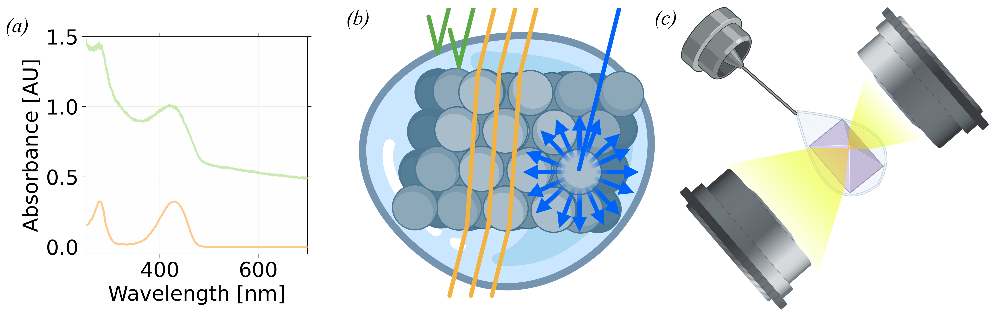
\includegraphics[width=\textwidth]{images/Spectroscopy/icOS_toolbox_Fig.1.pdf}
    \hfill
    \caption{Optical phenomena occurring in a protein crystal. \textbf{(a)} Comparison of an in solution (orange curve) and in crystallo (green curve, with a non-null, non-flat baseline) AS spectra. \textbf{(b)} Representation of several optical phenomena occurring in crystals that can contribute to the background: reflectivity (green rays), refraction (orange rays), which does not per se cause photon loss, and Rayleigh scattering (blue rays) which causes photon loss \textbf{(c)} Schematic representation of a single crystal microspectrophotometry setup. The crystal is mounted in a loop and surrounded by its mother liquor. The focal cones of the upstream (top-right, focussing the incident beam) and downstream (to the spectrophotometer, bottom-left) objectives are shown in yellow. The downstream focal cone is larger than the upstream one to mitigate the displacement of the focal point effect described in \cite{vonstettenCrystalloOpticalSpectroscopy2015}.}
    \label{fig:toolbox_phenomena}
\end{figure}
\subsection{Focal spot displacement}

The light beam used for in solution AS is collimated, whereas it must be focussed on the crystal for \textit{ic}AS. Refraction of light at the interfaces of both the crystal and its mother liquor displaces the focal point of the objective, contributing to photon loss \parencite{vonstettenCrystalloOpticalSpectroscopy2015}. This effect artificially increases the measured optical density in \textit{ic}AS across the whole spectrum with a ‘flat baseline’ (Fig. \ref{fig:toolbox_phenomena} (a)). This effect can be mitigated by choosing an optical fibre with a larger diameter for the downstream objective than for the upstream objective, thereby increasing the downstream focal cone and catching most stray refracted photons (Fig. \ref{fig:toolbox_phenomena} (c)). 

\subsection{Spectral anisotropy}

The anisotropic properties of protein crystals also cause spectral artefacts. Photons are maximally absorbed when their electric vector (polarisation) is parallel to the dipole transition moment of a chromophore \parencite{eaton16PolarizedAbsorption1981}. In a solution with randomly-oriented chromophores, this does not matter, and photons polarised in any direction are absorbed with an equal probability. This is no longer true in protein crystals, because the chromophores are oriented along a restricted number of directions as a result of the crystallographic and non crystallographic symmetry axes \parencite{eatonSingleCrystalSpectra1968}. As a consequence, protein crystals exhibit different extinction coefficients depending on crystal orientation with respect to the incident light beam \parencite{eatonSingleCrystalSpectra1968}, thus breaking the Beer-Lambert law. An extreme example of optical anisotropy can be observed for the Orange Carotenoid protein (OCP), where the two carotenoid chromophores are positioned almost parallel to each other in the asymmetric unit \parencite{kerfeldCrystalStructureCyanobacterial2003}. If observed through a polarised filter, OCP crystals appear totally colourless in some orientations and orange in others, in other words, the crystals are birefringent \parencite{kerfeldCrystalsCarotenoidProtein1997}. While OCP is an extreme example, all protein crystals exhibit anisotropic optical properties to varying degrees. Because the protein crystal also acts as a light polariser, the shape of an \textit{ic}AS spectrum will depend strongly on the crystal orientation. In order to record quantitative absorbance in crystals, the incoming and downstream light must be polarised along one of the symmetry axes of the crystals. In this case the probability of absorption is equal for all photons and the Beer-Lambert law is again applicable \parencite{mozzarelliProteinFunctionCrystal1996}. 

\subsection{Artefacts associated with fluorescence}
Other phenomena can unfortunately not be reliably modelled and corrected. Owing to the density of fluorophores in protein crystals (including aromatic amino acids), a significant part of the absorbed light will generate fluorescent photons, some of which are collected by the measuring objective, creating negative features in the absorption spectrum (Fig. \ref{fig:toolbox_correction}.(b), red spectrum) \parencite{vonstettenCrystalloOpticalSpectroscopy2015}. Conversely, when measuring fluorescence emission spectra, the focusing volumes of the cones for both the excitation light and the measured signal need to be carefully chosen to prevent the so-called ‘self-absorption’ phenomenon leading to apparent red shifts of emission maxima \parencite{barrosCrystalStructurePlant2009,vonstettenCrystalloOpticalSpectroscopy2015}. 

\section{Correction of \textit{in crystallo} UV-vis absorption spectra in the \textit{ic}OS toolbox}
The exemplar spectra analysed here have been recorded on various instruments on beamlines at the European Synchrotron Radiation Facility (ESRF) or on offline setups nearby: the \textit{ic}OS Lab at the ESRF \parencite{vonstettenCrystalloOpticalSpectroscopy2015} or the CAL(AI)²DOSCOPE at the Institut de Biologie Structurale (IBS) \parencite{byrdinCALAI2DOSCOPE2016}. The CAL(AI)²DOSCOPE has been specifically, but not exclusively, designed for the study of fluorescent proteins \parencite{dezitterMechanisticInvestigationMEos4b2019,dezitterMechanisticInvestigationsGreen2020}.


All the phenomena discussed above complicate the direct comparison of \textit{ic}AS data to in-solution AS data. Before an \textit{ic}AS spectrum is measured, the orientation of the crystal must be carefully chosen to minimise the effect of focal spot displacement, anisotropy and potentially fluorescence. Further, the contribution of Rayleigh scattering as well as that of remaining focal spot displacement and reflection must be modelled to allow \textit{ic}AS data recorded on different crystals to be compared. Here we present a workflow for these correction procedures. This python application is wrapped in a graphical interface, able to apply these corrections to \textit{ic}AS and in crystallo fluorescence spectra, as well as analyse and compare spectra and prepare publication-ready figures. 


Recording meaningful \textit{ic}OS data with minimal optical artefacts requires a detailed knowledge of the setup used and its limitations. Online spectroscopy setups are scarce and often only temporarily available for dedicated beamtimes. Live feedback on the quality and correction of recorded \textit{ic}OS data either directly at the beamline or at the \textit{ic}OS lab can make or break a beamtime, especially if the analysis depends on data from different crystals. To that end, we have developed a user-friendly graphical application (Fig. \ref{fig:toolbox_GUI} a) into which AS and fluorescence spectra can be loaded from a text format. Several types of background and data correction are available, each of them addressing a specific optical artefact. In addition, the \textit{ic}OS toolbox provides a tool for live kinetic analysis of the data (Fig. \ref{fig:toolbox_GUI} b). Finally, figures are generated using the wxmplot package \parencite{newvilleNewvilleWxmplot2024}, and can be fully customized to reach publication quality (Fig. \ref{fig:toolbox_GUI} c).  The corrected data can be saved to ASCII format. This software is already deployed at the \textit{ic}OS Lab of the ESRF (HR2000+ or QE65Pro spectrophotometer (Ocean Optics), spectra recorded using SpectraSuite (Ocean Optics)), on the TR-\textit{ic}OS instrument \parencite{engilbergeTRicOSSetupESRF2024} (AvaSpec-ULS2048CL-EVO-RS-UA spectrophotometer (Avantes), spectra recorded using AvaSoft v 8.11 (Avantes)), as well as on the BM07-FIP2 online microspectrophotometry setup (QE65Pro spectrophotometer (Ocean Optics), spectra recorded using OceanView (Ocean Optics)) and the CAL(AI)²DOSCOPE setup at the IBS. It is also available for offline use at \url{https://github.com/ncara/icOS} and has been adapted to process solution data from JASCO spectrophotometers as well as online \textit{ic}AS data recorded on beamline I24 at Diamond Light Source \parencite{roseSpectroscopicallyValidatedPHdependent2024}. It can also be used to treat data recorded on solutions and on small molecule crystals.


\begin{figure}[H] %bt!]
    \centering
    \noindent 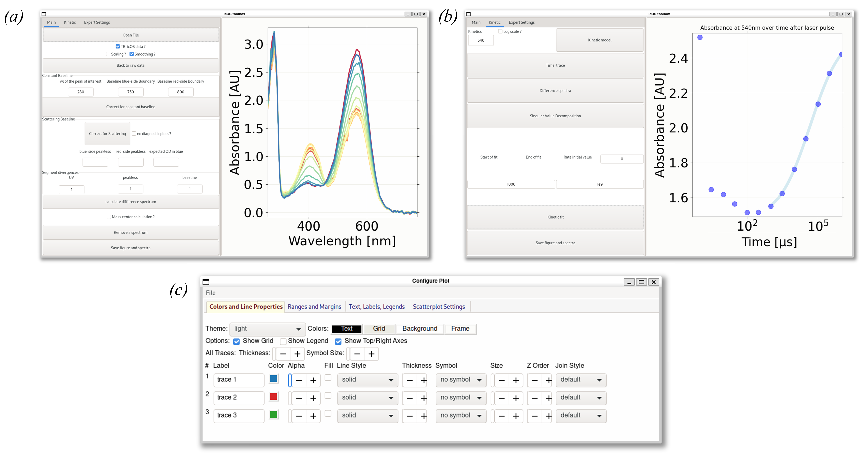
\includegraphics[width=\textwidth]{images/Spectroscopy/icOS_toolbox_Fig.2.pdf}
    \hfill
    \caption{The \textit{ic}OS app GUI (\textit{a}) main panel (\textit{b}) kinetic analysis panel (\textit{c}) figure customization panel.}
    \label{fig:toolbox_GUI}
\end{figure}

\subsection{Levelling and scaling: correcting for the displacement of the focal point and crystal size}

Various phenomena previously described contribute to uniformly raising the baseline of an \textit{ic}AS spectra (Fig. \ref{fig:toolbox_phenomena} (a); Fig. \ref{fig:toolbox_correction} (a)). This is easily corrected, provided the spectrum features a region devoid of absorption. The average of absorption in this band is subtracted from each spectrum to bring them onto a common baseline (Fig. \ref{fig:toolbox_correction} b). In the app, this function is called “constant-baseline correction”. 


Unlike solutions in spectroscopy cuvettes, the shape of protein crystals is irregular: they present an optical path of varying depth. The concentration of absorbing species in protein crystals cannot be adjusted, and their optical density is anisotropic. Therefore, the amount of absorbing material traversed by the incoming light depends on the size and shape of a crystal, but also on the orientation of the crystal with respect to the light path. Spectra from different crystals or orientations should therefore be scaled based on a conserved absorption peak. The choice of a peak can be inferred from prior knowledge in solution data. 




\begin{figure}[H] %bt!]
    \centering
    \noindent 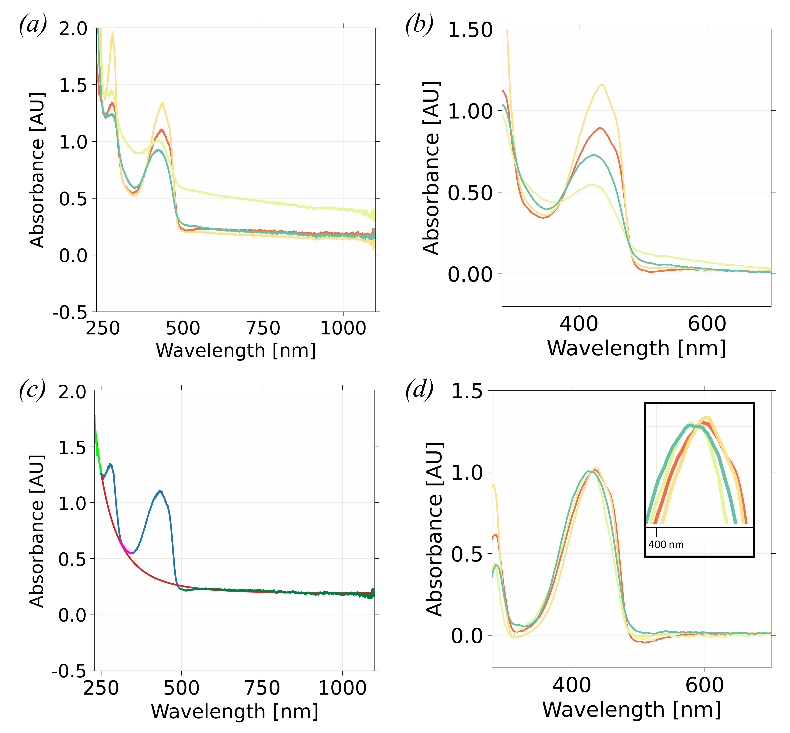
\includegraphics[width=\textwidth]{images/Spectroscopy/icOS_toolbox_Fig.3.pdf}
    \hfill
    \caption{\textit{ic}AS of a variant of different crystals of the Cerulean fluorescent protein, at several points after they were soaked from pH 8.0 to pH 4.0 (\textit{a}) without correction (\textit{b}) after constant baseline correction and smoothing (\textit{c}) example of the scattering baseline correction, with the three segments used to fit the baseline in dark green (red-side baseline), magenta (peak-less segment) and near-UV segment (lime) (\textit{d}) Scattering corrected spectra. The correction separates the red and yellow spectra from the dark green and light green spectra. The inlet shows the detail of the peak summit, 390 nm to 450 nm.}
    \label{fig:toolbox_correction}
\end{figure}

\subsection{Scattering and reflection correction}

Protein crystals are dense optical media, often surrounded by a layer of solution. The amount of light lost to reflectivity at each interface depends on the refraction indices of the crystal and its mother-liquor which are a function of the wavelength. The contribution of reflectivity to the baseline can be estimated by the Fresnel equations. Assuming the spectra have been recorded in the optimal direction, and the angle of incidence of the incoming light is mostly normal, the share of light lost to reflectivity (\textit{R}) as a function of the refractive indices (\textit{ni}) of both media at the interface corresponds to 


\begin{equation}\label{eq:reflection}
R = \left(\frac{n_1 - n_2}{n_1 + n_2}\right)^2
\end{equation}


The refractive index of each medium can be expressed as a function of the wavelength (\textlambda) with the Cauchy Equations, where \textit{a} and \textit{b} are material specific coefficients that can be derived by fitting to the measured refractive index at different wavelengths, but are used here as parameters fitted against the data to estimate the contribution of reflectivity.
\begin{equation}\label{eq:refraction_index}
n_1 =a + \frac{b}{{\lambda^2}}
\end{equation}
Therefore the contribution reflectivity to the baseline distortion of an \textit{ic}AS spectrum can be estimated as 
\begin{equation}\label{eq:reflection_f_wavelength}
R(\lambda) = \left(\frac{a+\frac{b}{\lambda^2} - c-\frac{d}{\lambda^2}}{ a+\frac{b}{\lambda^2}  + c+\frac{d}{\lambda^2}}\right)^2
\end{equation}





Where a, b, c and d are parameters which will be fitted against the data.
The amount of visible range photons Rayleigh scattered by a protein crystal scales inversely proportional to \textlambda \textsuperscript{4} \parencite{calvertGlossaryAtmosphericChemistry1990}


\begin{equation}\label{eq:rayleigh}
\sigma(\lambda) = \frac{a}{{\lambda^4}}
\end{equation}


The combined contribution of reflectivity and Rayleigh scattering to the baseline can thus be estimated as a function of the wavelength using  


\begin{equation}\label{eq:modeling_background}
    Full\ baseline(\lambda) = \left(\frac{a+\frac{b}{\lambda^2} - c-\frac{d}{\lambda^2}}{ a+\frac{b}{\lambda^2}  + c+\frac{d}{\lambda^2}}\right)^2 + \frac{e}{{\lambda^4}}
\end{equation}


In this model parameters a, b, c, d and e are fitted against the data points from three non-absorbing (supposed baseline) segments of the spectra via the least-square minimization method (lime, magenta and dark green segments in Fig. \ref{fig:toolbox_correction} (c)). Ideally, two of these segments are on either side of the recorded range (Fig. \ref{fig:toolbox_correction} (c)), one where Rayleigh scattering is respectively strongest (lime, Fig. \ref{fig:toolbox_correction} (c)), and the other where it is weakest (dark-green, Fig. \ref{fig:toolbox_correction} (c)). Because the UV segment is sometimes unreliable (loss of signal through the optics visible in Fig. \ref{fig:toolbox_TRicOS} (a)), a third segment, between the UV range and the absorption peak of interest (magenta, Fig. \ref{fig:toolbox_correction} (c)), is also used to fit the baseline model (plotted in red in Fig. \ref{fig:toolbox_correction} (c)). Additionally, a divergence factor (always positive, 1 by default) can be applied to decrease the weight of each segment in the fit of the scattering baseline (Fig. \ref{fig:toolbox_GUI} (a)). This divergence factor should be inversely proportional to the length of its segment and increased if the segment is less reliable. The segments on the left and right side of the region of interest are user inputted (Fig. \ref{fig:toolbox_GUI} (b)). If the absorbance does not go back to the baseline between the absorption peak of interest and the UV-range, a percentage of the maximum absorbance peak can be supplied to create a constant offset between the fit and the absorbance (Fig. \ref{fig:toolbox_GUI} (a)). A diagnostic plot is generated for each spectrum. In this diagnostic plot, segments used in the fit are coloured (lime, magenta and dark-green), and the fit baseline is overlaid (red) for assessment of the background correction quality (Fig. \ref{fig:toolbox_correction} (c)). The range and divergence factor of each segment should be adjusted so that the fit baseline is superposed onto the segments selected to fit against. Finally, the modelled contribution of both phenomena as well as the flat baseline can be subtracted from the raw spectrum, effectively bringing the baseline to 0 (Fig. \ref{fig:toolbox_correction} (d)). 

The data shown in Fig. \ref{fig:toolbox_correction} correspond to absorption spectra of crystals of the Cerulean Fluorescent protein grown at neutral pH and cryo-cooled at various delays after they were soaked in acidic pH buffer (behaviour of Cerulean at neutral and low pH is characterised in \parencite{gotthardChromophoreIsomerStabilization2017a}).  For these spectra, the background correction reveals a blue-shift and a change of shape of the main absorbance peak and allows grouping of spectra into two distinct families: red and yellow with a two-shouldered shape peak at 430 nm, and green and dark green spectra with a Gaussian shaped peak centred at 425 nm as well as a change of shape from the initial one peaked, two-shouldered shape (red and yellow spectra, Fig. \ref{fig:toolbox_correction} d) to a blue-shifted peak without shoulders as time goes on (green spectra, Fig. \ref{fig:toolbox_correction} d). The two families of spectra were not so easily discernible in the raw data.

In some cases, such as X-ray induced baseline alterations \parencite{boltonRedoxSwitchAllows2024}, the standard baseline model does not perform well. The user can then choose between pure Rayleigh scattering (no reflectivity) and a custom \textlambda \textsuperscript{-n} which, in our experience, has empirically performed well for X-ray induced optical artefacts. 

\subsection{Smoothing}
Depending on the shape and optical density of the crystal, the signal to noise ratio (SNR) of \textit{ic}AS data can sometimes be poor. Identification of correct peak positions and centre of mass can benefit from a noise removal step. Both a Savitzky-Golay filter (in this case, fitting of a third-degree polynomial function over windows of 21 data-points) and a rolling average are available as options in the ‘expert features’ tab for the smoothing of \textit{ic}OS data.  


\section{Kinetic \textit{ic}OS analysis}

The \textit{ic}OS lab allows recording of kinetic series on millisecond to minutes time-scales for fluorescence decay analysis, slow protein dynamic events, or deriving a photoreduction dose for an X-ray sensitive species on-line \parencite{boltonRedoxSwitchAllows2024} and off-line \parencite{aumonierSlowProteinDynamics2022}. A recent instrumentation update now allows off-line recording of time-resolved \textit{ic}AS down to the µs range \parencite{engilbergeTRicOSSetupESRF2024}. Depending on the recording procedure, different data-processing pipelines should be used. 

\subsection{Spectral series: the case of time-resolved or dose-resolved data}

In an ideal case, a kinetic series is recorded on the same crystal at the same angle and position. Even then, slight, achromatic variations of the baseline can still be observed due to fluctuations of the cryo-stream or humidifier \parencite{sanchez-weatherbyImprovingDiffractionHumidity2009}, or variation in intensity of the pulsed white lamp in the case of the TR-\textit{ic}OS instrument at ESRF. In this ideal case, only the constant baseline correction described in § 2.1.1 is needed, and potentially a smoothing of the data (Fig. \ref{fig:toolbox_TRicOS} (a), (b)). The example shown in Fig. \ref{fig:toolbox_TRicOS} depicts the correction, smoothing (Fig. \ref{fig:toolbox_TRicOS} (b)) and calculation of a series of difference absorption spectra (Fig. \ref{fig:toolbox_TRicOS} (c) of a bacteriorhodopsin (BR) crystal. These corrections allow precise assessment of the timescale of the rise of the characteristic M state 400-nm peak \parencite{efremovTimeResolvedMicrospectroscopySingle2006} and drop in absorbance of the main 600-nm peak as the sample returns to the ground state. 

\begin{figure}[H] %bt!]
    \centering
    \noindent 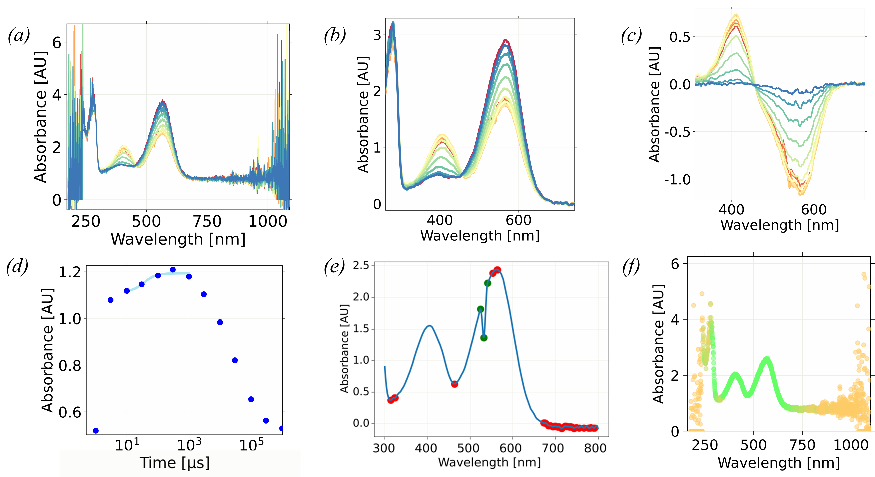
\includegraphics[width=\textwidth]{images/Spectroscopy/icOS_toolbox_Fig.4.pdf}
    \hfill
    \caption{Time-resolved \textit{ic}OS data in the GUI (\textit{a}) series of time-resolved AS, collected on Bacteriorhodopsin (BR) crystals, after exposure to a  560-nm ns laser pulse, raw. (\textit{b}) Spectra constant-baseline corrected and smoothed, with laser trace removed.  (\textit{c}) Series of \textit{light – dark} difference spectra. For panels a-c the colour ramps from red to blue as the reaction progresses, spectra are recorded at 3 µs, 10 µs, 30 µs, 100 µs, 300 µs, 1 ms, 3 ms, 10 ms, 30 ms, 100 ms, 300 ms and 1s. (\textit{d}) Absorption at 400 nm (M state of BR), integrated from the spectra represented on panel (\textit{b}). (\textit{e}) Absorption spectrum of the spectrum recorded 3 µs after the actinic laser pulse, in which all dips in absorbance are identified by red dots. The largest dip in absorbance is identified by green dots, and corresponds to the tail of the nanosecond laser pulse. (\textit{f}) Confidence plot of the 300 µs TR-\textit{ic}OS spectrum, each data point is plotted from orange (low confidence) to green (good confidence).}
    \label{fig:toolbox_TRicOS}
\end{figure}


\subsubsection{Time-trace and Constant fitting}
Spectral regions associated with key species can be identified. Their absorbance can be extracted and plotted over time in the \textit{ic}OS toolbox GUI to create a time-trace (Fig. \ref{fig:toolbox_TRicOS} (\textit{d})). 
Provided these prerequisites are met, a kinetic model can be fitted to the data points. The \textit{ic}OS toolbox currently allows the fit of a mono-exponential decay or rise, as well as the Hill Equation. The produced reaction rate constant provides an estimation of an intermediate-state lifetime and can be used to plan a TR-MX experiment. Finally, rate constant fits are particularly suited to the detection of artefactual reaction pathway caused by non-linear multi photon absorption events 
\parencite{doTwophotonAbsorptionPhotoionization2023,engilbergeTRicOSSetupESRF2024,barendsInfluencePumpLaser2024,bertrandStructuralEffectsHigh2024}. 

\subsubsection{Laser dent removal}

Because of the duration of integration of the spectrophotometer, the tail of the nanosecond laser pulse used to initiate a reaction in a crystal can also contribute to the absorption spectrum, in the form of a negative dip, or dent in the absorption spectrum (Fig. \ref{fig:toolbox_TRicOS} (\textit{e})). To identify this the second derivative of the absorption spectra is calculated. The local minima identify the absorption dips, as well as their edges. The largest absoption dip (in amplitude) marks the contribution of the nanosecond laser to the spectrum, while all other dips are marked by red dots. The data points corresponding to the contribution of the laser are removed. For spectra of subsequent time-points, only the main dent in the area of the previously detected laser dent is marked, and the corresponding points are also removed.

\subsubsection{Confidence score}

Absorbance is calculated by comparison to a reference signal as I0, but the emission spectrum of the polychromatic light sources used for \textit{ic}OS often exhibit low photon count regions. These regions typically exhibit noisy peak-like features which might appear meaningful to the untrained eye. In order to easily assess the validity of a feature, we implemented a confidence-score based on the photon count in the reference signal for each measurement. This confidence score is visualised as a colour scale from blue (trustworthy) to red (untrustworthy) via the ‘expert features’ panel (Fig. \ref{fig:toolbox_TRicOS} (\textit{f})). When raw photon counts are available, a confidence score is calculated to identify features of a spectrum that might originate from a low count in both the I0 blank signal and the I signal. 

\subsubsection{Singular Value Decomposition}

When a series of spectra is available, it can be analysed with Singular Value Decomposition (SVD), to provide additional insights into time or dose dependent behaviour. SVD is an algebra based analysis technique which has been widely used in the fields of time-resolved spectroscopy \parencite{henryUseMatrixMethods1997,henrySingularValueDecomposition1992}. Briefly, the aim of SVD is to determine a minimal set of basis spectra, which can be linearly combined to make up any of the observed spectra across the series. It consists of the decomposition of a matrix, A containing the observed spectra in rows, in chronological order. This input-matrix traditionally contains light – dark difference spectra to remove unchanging features. A is Eigen-decomposed into U, S and V, respectively containing the basis spectra (right Singular Vector, rSV), weighing factors of each feature from U (Singular Values, SV) and scalars weighing each basis spectra from U to recreate the observed spectra from A (left Singular Vector, lSV). This corresponds, in the case of a time-resolved series of spectra, to a decomposition into basis spectra and time-evolution of these basis spectra over the studied time-range. 

\subsection{Serial Time-resolved \textit{in crystallo} UV-visible absorption spectroscopy}
When a reaction is too slow or irreversible in crystallo, only one measurement per crystal is possible. For measurements performed on the same crystal, only the constant baseline correction is needed, to account for variation in surrounding medium refraction index or flash lamp pulse intensity. After this correction, a light-dark difference spectra can be calculated for each time point. In a series of spectra (recorded on different crystals) the height of the difference peaks is influenced by the thickness of each crystal, meaning a scaling scheme has to be applied before comparison. This enables pairwise analysis if the correction of crystal shape derived baseline artefacts proves impossible. Here, once bands of interest are identified in the difference spectra, the area under the bands of interest can be integrated and plotted against time, creating a serial-\textit{ic}OS time-trace (Fig. \ref{fig:toolbox_TRicOS} (\textit{d})). Because of all the phenomena described in § 2, it is challenging to translate an integrated absorbance value into the occupancy of a reactive intermediate in this case. However, a kinetic model can be fitted to this set of points, providing a precise estimation of a reaction intermediate rise and decay time in crystallo.

\section{Dos and Don'ts}

The wavelength, or wavelength range chosen for the extraction must be devoid of any saturation (evidenced by noisy, truncated peak summits), but also reasonably high confidence (see Fig. \ref{fig:toolbox_TRicOS} (\textit{f})). 
Ideally, only the tracked species should absorb in chosen region, so that a change of absorption can be solely attributed to a change in occupancy of the tracked species. Choosing a good wavelength for the investigation of a RIS-state can mean choosing to minimise noise and contamination over maximising the intensity of the signal.


\section{Conclusion}
In this article, we have described the optical phenomena altering \textit{ic}OS data and presented various steps to treat these in subsequent data analysis. We have presented a workflow to analyse \textit{ic}OS data, and finally, set of tools which can be used to achieve each step. A graphical user interface is supplied with these tools to allow the analysis of \textit{ic}OS data directly at the beamline or on the \textit{ic}OS platform at ESRF so that the most analysis can be done during a diffraction beamtime. The \textit{ic}OS app has already been successfully used in several TR-MX projects, including by non-supervised users. The app, as well as instructions on how to use it can be found at \url{https://github.com/ncara/icOS}.

\section*{Acknowledgements}
The authors thank Sylvain Engilberge, Samuel Rose, Sergei Bukhdruker, Mohammad Chorfa and Alexander Sprott for fruitful interaction and requests. Christoph Mueller-Dieckmann and David von Stetten are also acknowledged for insightful discussion and advice. The ESRF structural Biology Group and the Pearson Research Group are acknowledged for their continuous support.


\chapter{On-line spectroscopy - the FutA example}\label{chap:online-microspec}
\noindent The paper will not be reproduced in its entirety, only my contribution will be discussed, with elements of context. 

\vspace{10mm}

The toolbox described in Chapter \ref{chap:toolbox} was of particular use during on-line spectroscopy experiments on BM07-FIP2. There, it was used to instantly derive a reaction rate from spectroscopic measurement, to identify any possible perturbation (drop of the humidity, decay of the flux in the excitation light source, slippage of the crystal).

Cyanobacteria of the ecotype \textit{Prochlorococcus} are the main contributors to global photosynthesis, fixing the same amount of carbon yearly that is produced by agriculture globally \parencite{hustonGlobalDistributionNet2009}. The photosynthetic proteins of \textit{Prochlorococcus} - and all phytoplankton - require iron for their electron transfer chains \parencite{ravenRoleTraceMetals1999}. Iron is extremely scarce in oceanic environments because it exists in its oxidised form and quickly precipitates to the ocean floor (where photosynthesis cannot happen, for lack of light) \parencite{wellsIronChemistrySeawater1995}. The bioavailability of iron is therefore one of the main limiting factors to the growth of cyanobacteria. Typically, cyanobacteria utilise several iron uptake systems, involving organic iron solubilisers, membrane transporter and cytosolic transporters. Members of the \textit{Prochlorococcus} have a reduced genome, as a trade-off for their extremely small size, which gives them an evolutionary advantage over other cyanobacteria in low-nutrient waters \parencite{billerProchlorococcusStructureFunction2015}. Consequently, they harbour only one gene, coding for one protein responsible for all of the functions listed above \parencite{rocapGenomeDivergenceTwo2003}. The protein, FutA, must bind both Fe(II) and Fe(III) to perform its functions. The study sought to identify the structural mechanism allowing this iron transporter to stabilise both redox forms of iron.  


When a protein crystal is exposed to X-rays, water, precipitant or other solvent molecules are radiolysed, releasing photoelectron \parencite{garmanRadiationDamageBiological2023}. Metals coordinated in proteins - and all other electron sinks - are reduced by these photoelectrons, thus altering the structure of the protein. This has been leveraged to activate redox enzymes at cryogenic temperatures \parencite{berglundCatalyticPathwayHorseradish2002,roseSingleCrystalSpectroscopy2022}. Expectedly, when the structure of FutA was first solved by X-ray diffraction, the crystal was partially bleached by the X-ray beam, turning from rust-coloured to burgundy. To derive the dose budget within which the coordination of the oxidised ion could be observed, \textit{in crystallo} spectroscopy under X-ray exposure was used. 

\section{On-line spectroscopy setup on BM07-FIP2}
\subsection{Geometry of the on-line microspectrophotometer}

Online micro spectrophotometry at beamline ESRF BM07-FIP2 uses 100-800 \textmu m optical fibre to connect a balanced deuterium-halogen lamp (Mikropack DH2000- BAL, Ocean Optics) to the upstream objective, while a 400-1000 \textmu m optical fibre connects the lower objective to a fixed-grating spectrophotometer equipped with a CCD detector (QE65 Pro, Ocean Optics) (Fig. \ref{fig:online_microspec_BM07}. For the FutA beamtime, spectra were acquired at 0.4 Hz (250 ms acquisition time averaged 10 times) on several crystals with a volume between \(160 x 70 x 50 \mu m^{3}\) and \(200 x 90 x 80 \mu m^{3}\). Crystals are oriented to optimize the signal-to-noise ratio of the spectra and maintained still during X-ray exposure (for reasons discussed in Chapter \ref{chap:toolbox} in a loop-mount using a humidity controller (HC-Lab, Arinax) \parencite{sanchez-weatherbyImprovingDiffractionHumidity2009}. Data analysis was carried out using the \textit{ic}OS toolbox (described in Chapter \ref{chap:toolbox}). Spectra were first baseline-corrected by subtraction of a constant corresponding to the average absorption between 800 and 880 nm. They were then smoothed using a Savitzky-Golay filter (parameters: 3rd order polynomial; 25-data point smoothing window).

\begin{figure}[H] %!ht]
\begin{center}
\noindent 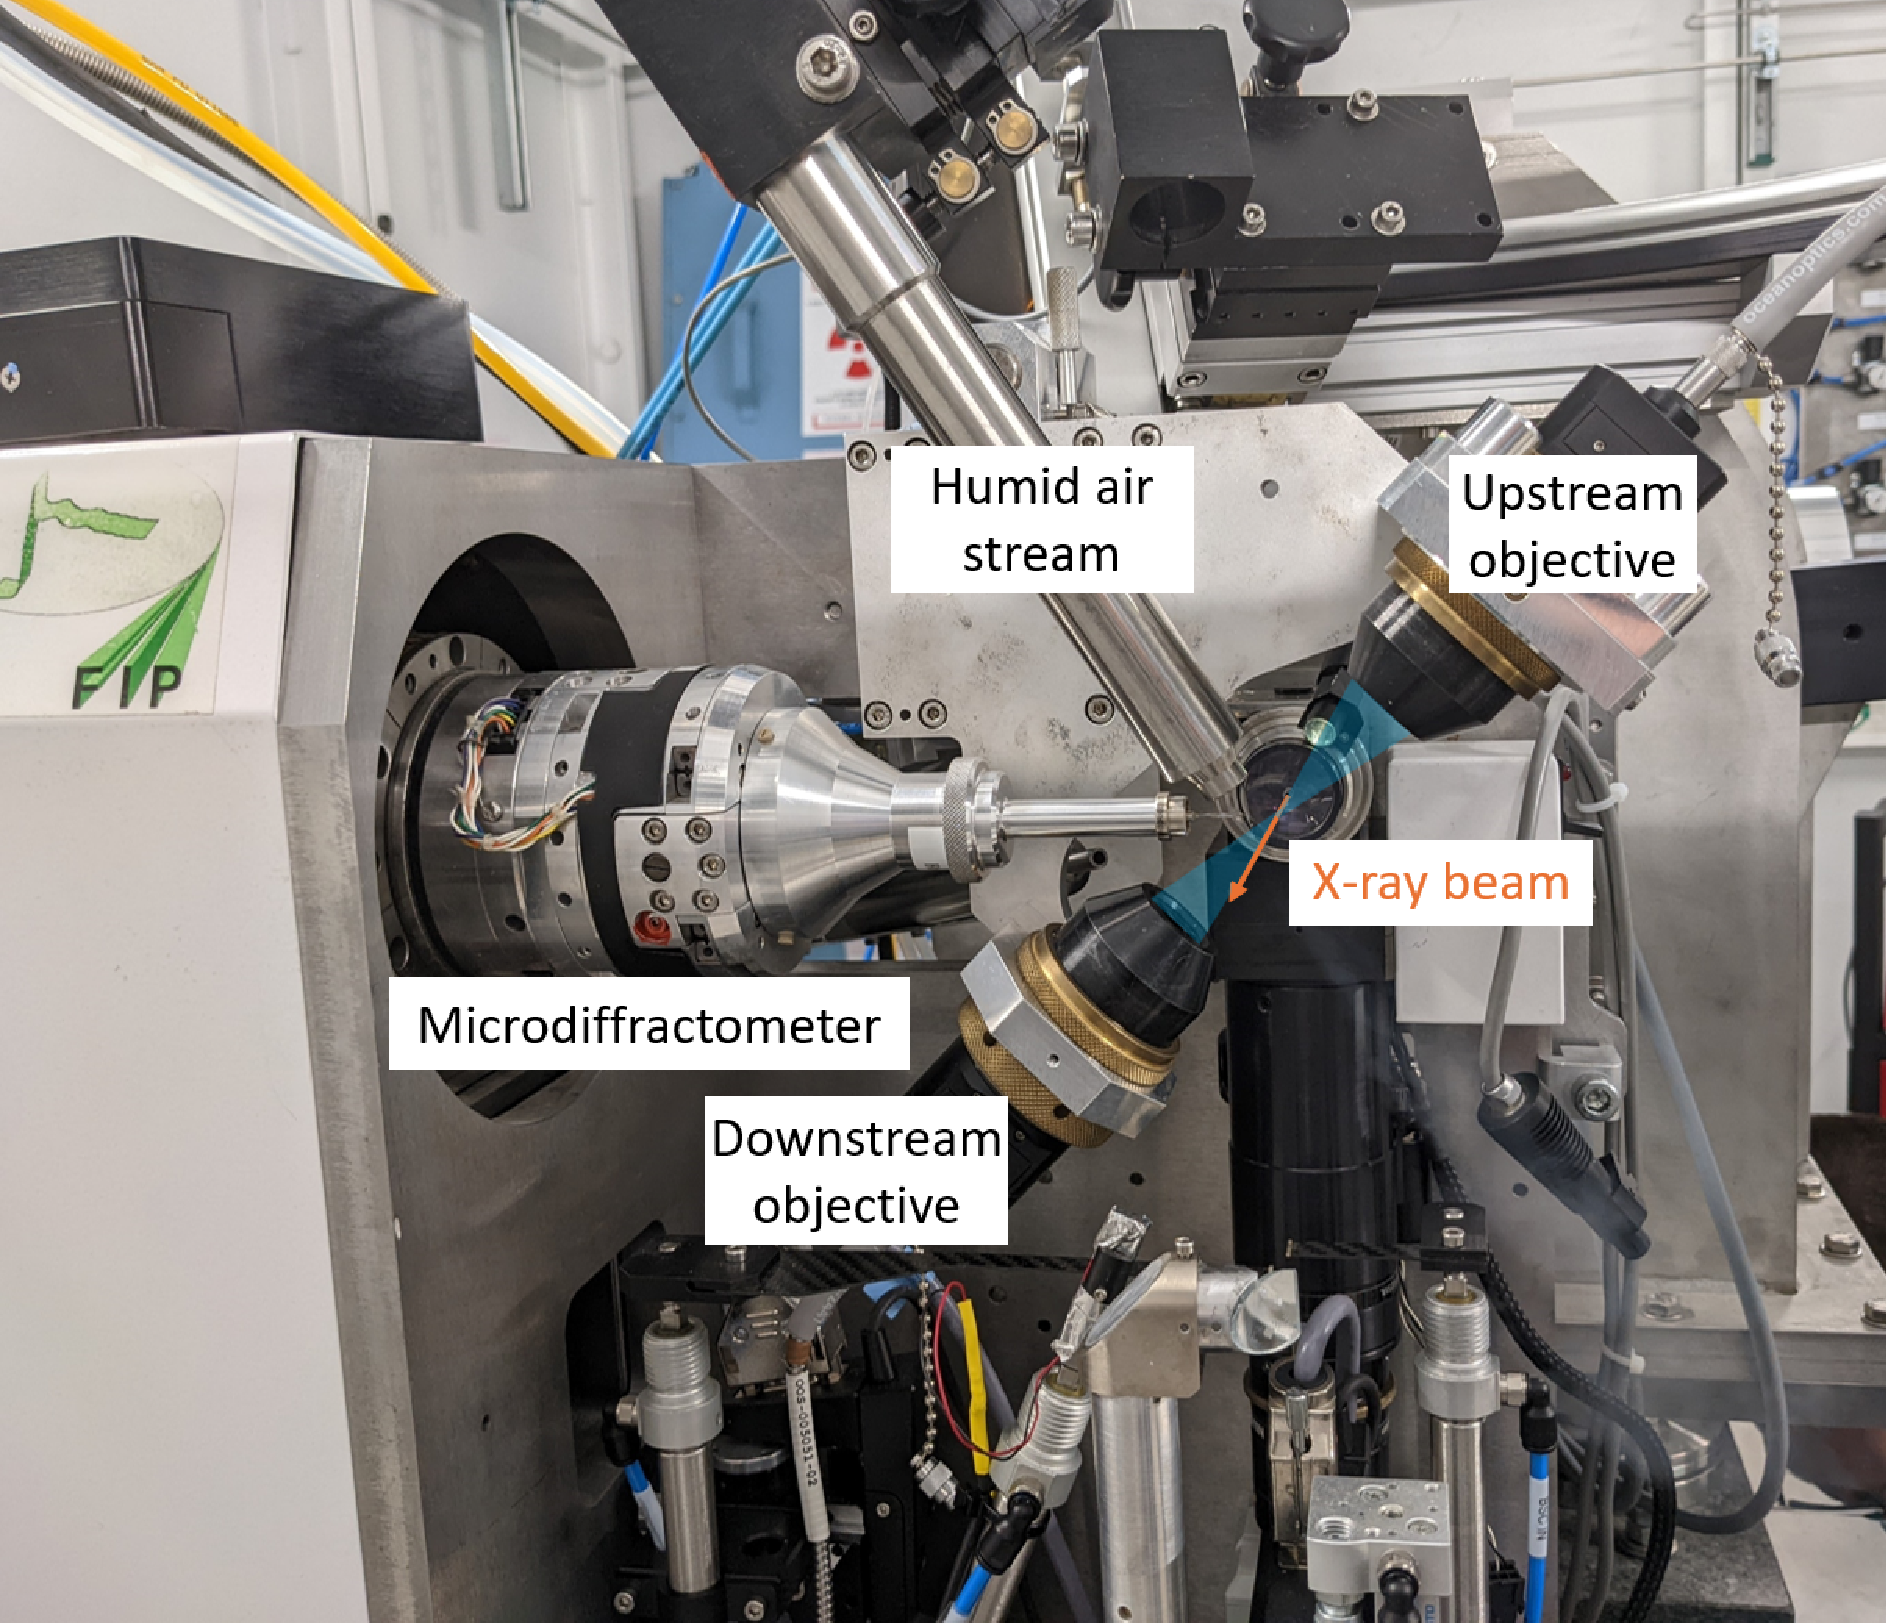
\includegraphics[width=0.8\textwidth]{images/Spectroscopy/geometry.pdf}
\end{center}
\caption{Geometry of the on-line spectroscopy setup of BM07. The deuterium-halogen lamp (Mikropack DH2000- BAL, Ocean Optics) lamp is focused by a first 4 \(\times\) demagnifying Schwarzschild objective (green) achromatically, onto the interaction point of the X-ray (focal volumes are represented in blue, the X-ray beam is represented by an orange arrow). The focal volume of the setup can be adjusted by changing the diameter of the optic fibres plugged into the upstream and downstream objectives. The downstream objective is connected to a microspectrophotometer (Ocean Optics, QE65 PRO). Crystals are manually mounted on the microspectrophotometer and maintained at cryogenic or room temperature.}
\label{fig:online_microspec_BM07}
\end{figure}

\section{Measuring the photoreduction rate of FutA}

\textit{in crystallo} spectra recorded on the beamline, during diffraction have been used extensively to characterise redox species and correlate them with diffraction structures, but almost exclusively at room temperature \parencite{berglundCatalyticPathwayHorseradish2002, beitlichCryoradiolyticReductionCrystalline2007,mcgeehanColouringCryocooledCrystals2009, uenoLowdoseXrayStructure2019}. Therefore, the photoreduction dose rate of FutA was first investigated with on-line spectroscopy on a crystal cryocooled and maintained at 100K. The Fe(III) absorption peak (\textlambda max = 438 nm) \parencite{orvilleStructuresCompetitiveInhibitor1997} of the absorption spectrum of a FutA crystal progressively decays on incident X-ray irradiation at a synchrotron beamline (Fig. \ref{fig:FutA_CT_RT} (\textit{c})). X-ray-induced light-absorbing species raise the baseline of the spectrum in the blue section of the spectrum, therefore, the decay was sampled at 464 nm (red side of the main absorption peak). Upon photoreduction, the Fe(III) decays monoexponentially, at 35 \(\pm\) 0.3 kGy, half of the Fe(III) is gone, and at 85 \(\pm\) 9 kGy, 80 \% is gone (dose calculated with RADDOSE 3D \parencite{buryEstimateYourDose2018}. However, while the crystals were cryocooled for the initial spectroscopy experiment, attempts at characterising the reduced structure of FutA were carried out at room temperature (220 K) so that protein movements could happen. And, perhaps expectedly, the rapid dose rate measured at 100K did not match the rate of discolouration observed for crystals exposed to the beam at room temperature (Supplementary Figure \ref{supfig:supfig_FutA}), prompting us to measure the dose rate of photoreduction at room temperature, on crystals maintained under a humid air stream of controlled saturation \parencite{sanchez-weatherbyImprovingDiffractionHumidity2009}. As X-rays induce light-absorbing chemical species in the solvent that overlap with the Fe(III) iron-specific signal, the 620 nm wavelength was chosen to minimize the effect of this artefact and characterize photoreduction of the iron centre, plotting the absorbance against accumulated radiation dose (Fig. \ref{fig:FutA_CT_RT} (\textit{a})). Measuring five different crystals, we determined a much higher half-photoreduction dose of 128 \(\pm\) 21 kGy; the dose at which 80\% of the molecules had been photoreduced was 204 \(\pm\) 27 kGy (Fig. \ref{fig:FutA_CT_RT} (\textit{b})), which was more consistent with the discolouration rate of FutA crystals as datasets were recorded.

\begin{figure}[H] %!ht]
\begin{center}
\noindent 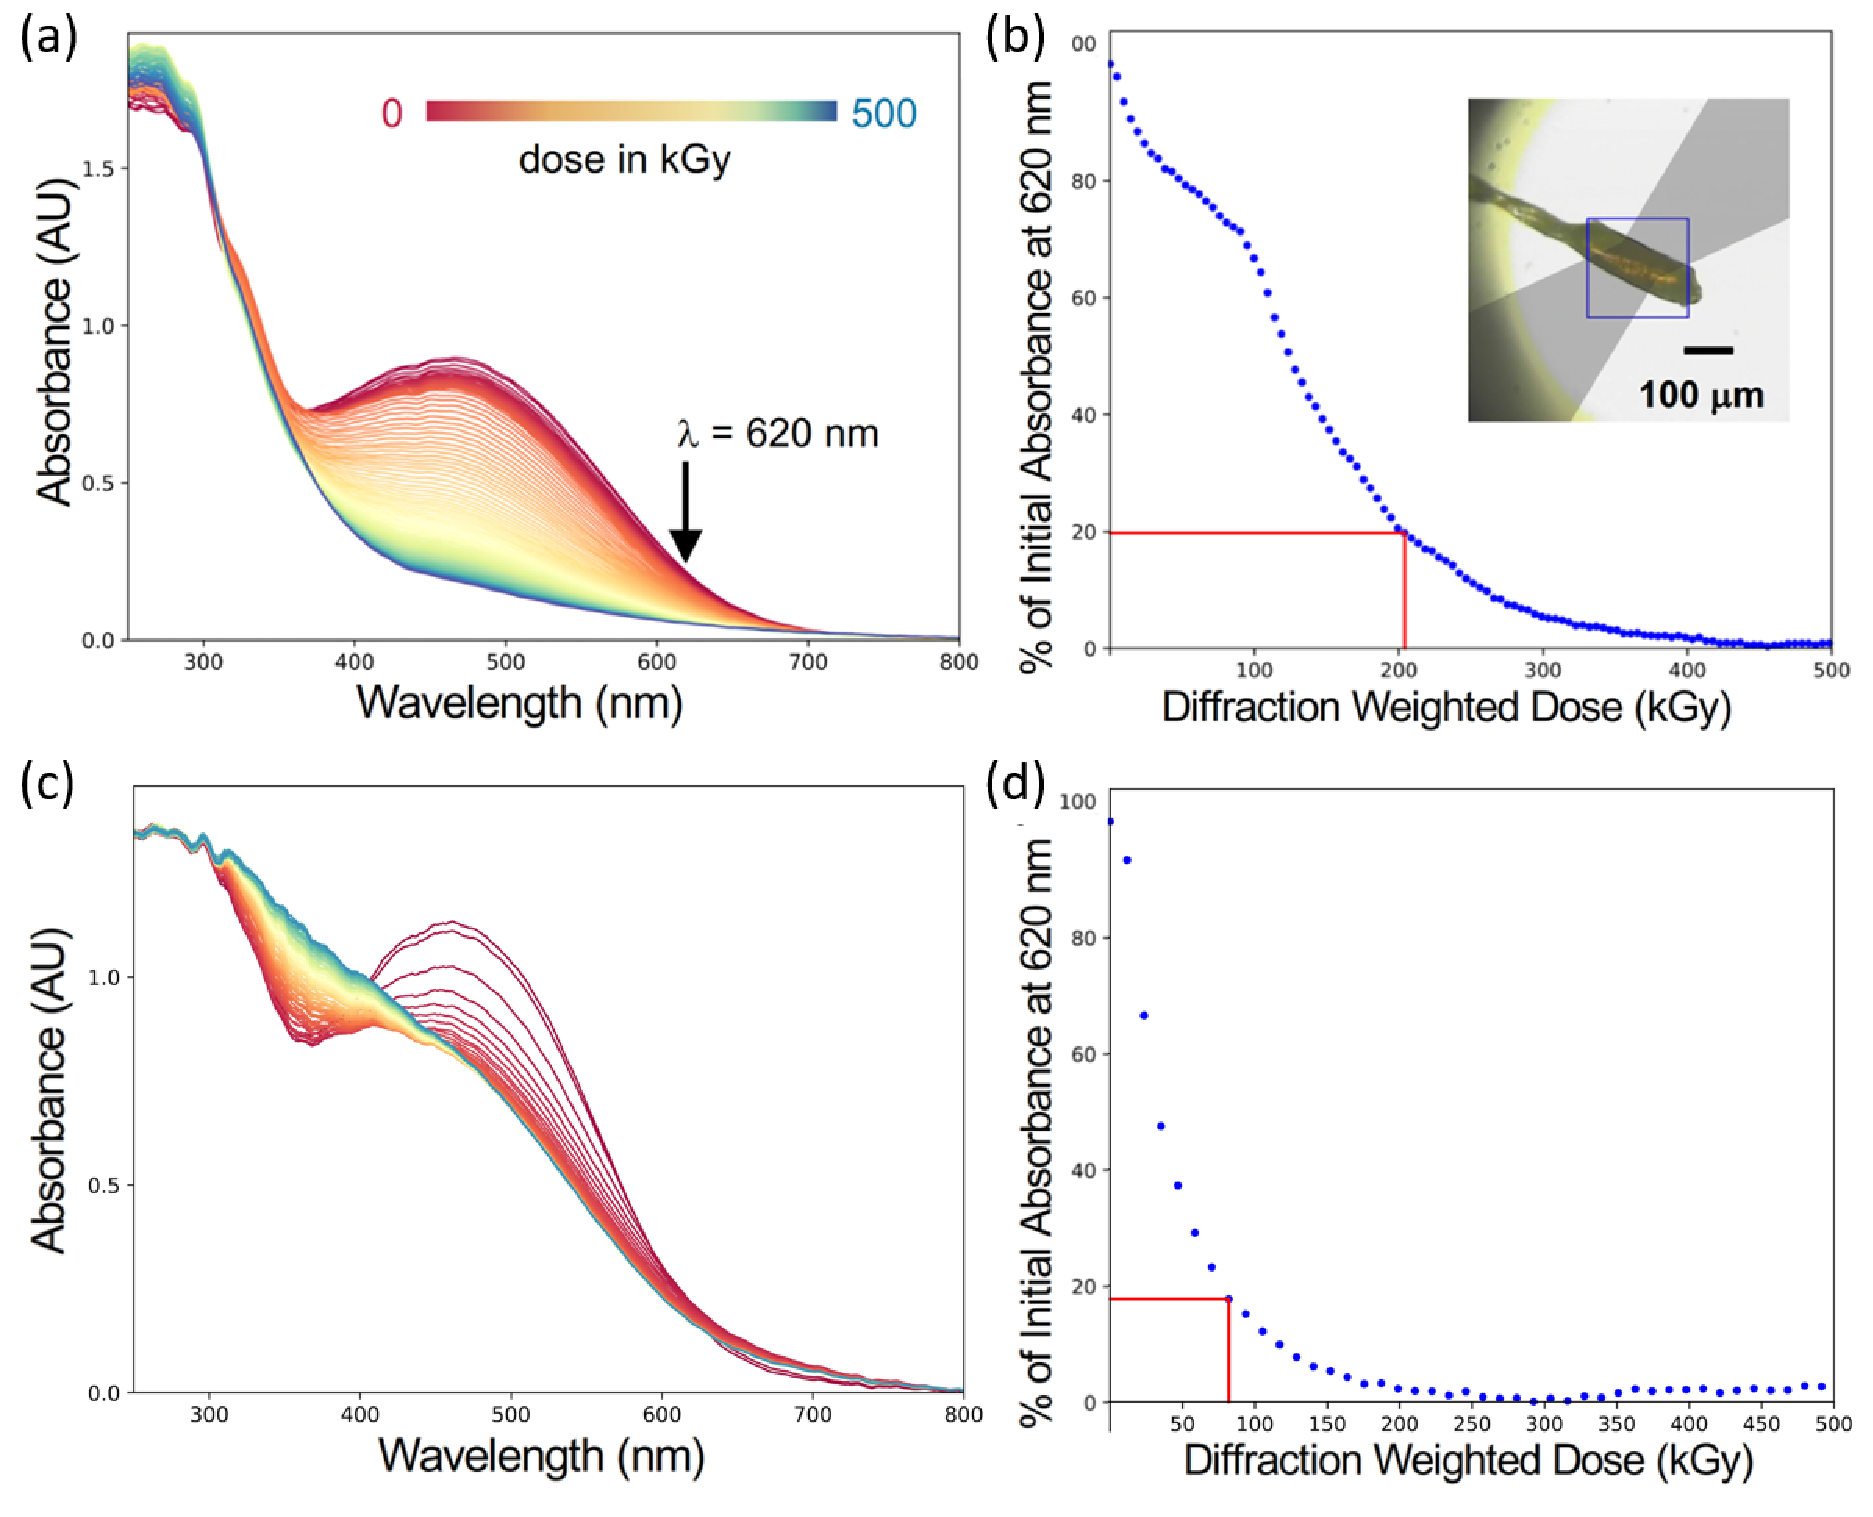
\includegraphics[width=0.8\textwidth]{images/Spectroscopy/FutA_ic_spectro_CT-vs-RT.pdf}
\end{center}
\caption{Photoreduction of iron in the FutA iron transporter, tracked via \textit{In crystallo} on-line spectroscopy. (\textit{a}) \textit{ic}AS spectra of FutA, collected at (220 K) during X-ray exposure, from 0 kGy (red) to 500 kGy (blue). Photoreduction over dose was assessed at a wavelength of 620 nm (arrow) to minimise the baseline distortion effect in the spectra blue wavelength range. (\textit{b}) Absorbance at 620 nm over dose decaying in two steps, with a half reduction dose of 128 \(\pm\) 21 kGy and an 80\% reduction dose of 204 \(\pm\) 27 kGy (red lines). The area of the crystal that was probed by the microspectrophotometry objectives' focal volume (indicated by the shaded triangles, on-axis view, in the top right insert) was completely exposed to the X-ray beam of BM07-FIP2 (depicted by the blue square representing the beam shape). (\textit{c}) \textit{ic}AS spectra of a FutA, collected at cryogenic temperature (100 K)  during X-ray exposure, from 0 kGy (red) to 500 kGy (blue) (\textit{d}) Decay of the absorbance at 464 nm (blue side of the main absorption peak of FutA) with a half reduction dose of 35 \(\pm\) 0.3 kGy, and an 80\% reduction dose of 82 \(\pm\) 9 kGy. (\textit{c}) and (\textit{d}) are not the initial 100 K spectroscopic measurement, but a latter, more resolved, reproduction of those initial results for better characterisation of the system at 100 K}
\label{fig:FutA_CT_RT}
\end{figure}

With the exact dose rate identified, intermediate species could be identified in dose-resolved structures of FutA. An experiment at the SACLA X-FEL could be scheduled to record a true oxidised structure and X-ray pump-probe intermediates (For a very nice discussion on the value of X-FEL radiation damage-free structures for the study of metalloproteins, see \cite{moreno-chicanoComplementarityNeutronXFEL2022}. 

\section{Conclusion}

Through this PhD, I developed and helped develop \textit{in crystallo} methods to help design TR-MX experiments, characterise caught reaction intermediates and guide the refinement of kinetic crystallography structures. 